\documentclass{article}
\usepackage{graphicx}
\graphicspath{ {/home/frank/git/Lido-Belvedere/specifiche_lido_Castiglione_Francesco_Paolo} }
\title{Gestione di un lido}

\author{Francesco Paolo Castiglione(0706826)}
\date{2020-2021}

\begin{document}
\maketitle
\section{Descrizione generale}
Il sistema fornisce le tipiche funzionalità che caratterizzano un lido balneare quali l'accesso, da parte dei clienti, ai servizi del lido, le funzionalità della biglietteria che permettono di visualizzare o creare le prenotazioni, le funzionalità della cucina che permettono di segnalare lo stato di avanzamento degli ordini ed infine le funzionalità del bagnino che permettono di controllare lo stato attuale di occupazione della spiaggia e controllare l'identità dei clienti prenotati per le rispettive postazioni. 

\section{Architettura del sistema}

Tecnologie utilizzate:
\begin{enumerate}
	\item Classi \texttt{Java Servlet} e \texttt{JSP} per l'accettazione di richieste \texttt{http}, per la costruzione della pagina web di risposta e per il processo di elaborazione e controllo dei dati inseriti dal client;
	\item \texttt{HTML}, \texttt{CSS},  \texttt{Javascript} e \texttt{Bootstrap 4} per la creazione e gestione dell'interfaccia utente;
	\item \texttt{Apache Tomcat} quale middleware per il deployment della web application;
	\item Database relazionale con DBMS \texttt{MySQL} per la memorizzazione dei dati, con corrispettivo connettore \texttt{JDBC} per interfacciarsi al DBMS tramite Java;
	\item \texttt{JDBCRealm} per l'autenticazione degli utenti;
	\item \texttt{JSON} come formato dati per lo scambio di dati fra server e client;
\end{enumerate}

\newpage
\section{Requisiti funzionali}

\subsection{Generali}
\begin{enumerate}
	\item La pagina principale mostra una schermata di benvenuto con immagini del lido e un menù per la navigazione del sito;
	\item In seguito al login l'utente viene reindirizzato alla pagina principale e il menù per la navigazione mostra le opzioni relative al ruolo dell'account in questione;
	\item Qualsiasi tipo di utente ha la possibilità di effettuare il logout;
	\item E' possibile registrare un account con ruolo di \texttt{User(Utente)};
\end{enumerate}

\subsection{Cliente}
In seguito al login, il cliente potrà accedere ai seguenti servizi:
\begin{enumerate}
	\item Prenotare una postazione per la giornata selezionata, in una specifica fascia oraria o per l'intera giornata di apertura;
	\item Visualizzare le prenotazioni effettuate con relativi dettagli ed eliminare le prenotazioni per date successive all'odierna;
	\item Visualizzare il menù e selezionare per ogni pietanza/bibita la quantità desiderata, che può essere modificata prima di completare definitivamente l'ordine;
	\item Visualizzare l'elenco delle ordinazioni e leggerne i relativi dettagli, fra i quali lo stato(ordinazione elaborata, pronta al ritiro, ritirata);
\end{enumerate}

\subsection{Biglietteria}
\begin{enumerate}
	\item Può effettuare prenotazioni a nome di un cliente;
	\item Può visualizzare l'elenco delle prenotazioni effettuate da tutti i clienti ed eliminare prenotazioni per date successive all'odierna;
\end{enumerate}

\subsection{Bagnino}
\begin{enumerate}
	\item Può visualizzare lo stato di occupazione della spiaggia;
	\item Può visualizzare le informazioni relative alla prenotazione cliccando sulla postazione occupata nella mappa della spiaggia 
\end{enumerate}

\subsection{Cuoco}
\begin{enumerate}
	\item Può visualizzare lo stato delle ordinazioni;
		
	\item Può cambiare lo stato delle ordinazioni, da \textit{in elaborazione} a \textit{pronta} a \textit{consegnata}
\end{enumerate}

\subsection{Modello dei dati}
\begin{center}
	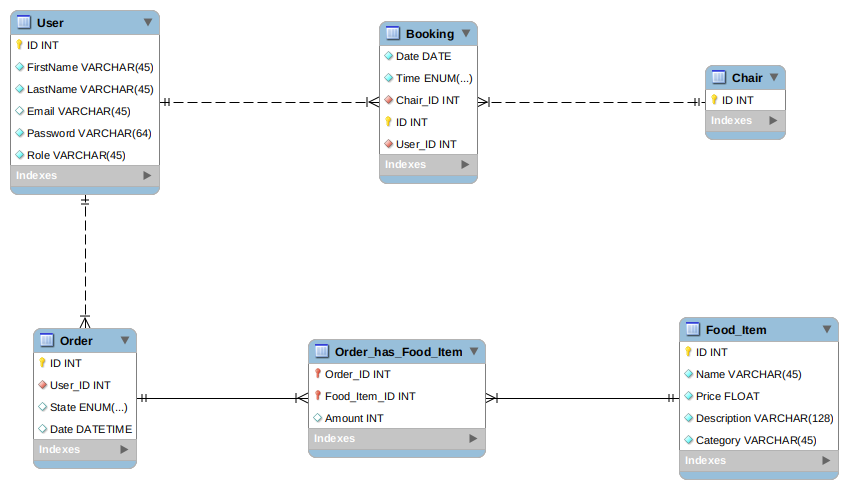
\includegraphics[scale=0.5]{dbmodel}
\end{center}


	
\end{document}